\documentclass[11pt]{article}

% ACL official style (github.com/acl-org/acl-style-files).
\usepackage[final]{acl}

\usepackage{times}
\usepackage{latexsym}
\usepackage[T1]{fontenc}
\usepackage[utf8]{inputenc}
\usepackage{microtype}
\IfFileExists{inconsolata.sty}{\usepackage{inconsolata}}{}
\usepackage{graphicx}
\usepackage{amsmath}
\usepackage{booktabs}
\usepackage{tabularx}
\usepackage{xcolor}
\usepackage{capt-of}

\newcommand{\code}[1]{\texttt{\small #1}}

\title{AquaGent: An Explainable Decision-Support Agent for\\Selecting Atmospheric Water Harvesting Technologies\\under Uncertainty and Constraints}

\author{Zainab Alameri \and Abubaker Baobaid \\
  Effat University, Jeddah, Saudi Arabia \\
  CS3081 Artificial Intelligence}

\raggedbottom
\begin{document}
\maketitle

% ---------------------------------------------------------------
\begin{abstract}
Collecting water from the air can help in dry areas, but there are different ways to do it and each one needs different conditions. A fog mesh needs fog and wind. A metal--organic framework (MOF) sorbent bed does not need fog, but it needs energy to release the water it holds. In this project we made AquaGent, a software agent that helps an operator decide between a Raschel-type fog collector, a MOF-303 sorbent bed, or no plan. The agent works in three steps. A Bayesian model uses the fog sensor reading, which can be wrong or missing, to estimate the chance of fog. A constraint satisfaction problem (CSP), solved with backtracking, removes plans that break safety, time, energy or weather limits. A score then ranks the plans that are left, and the operator accepts or rejects the result on a Streamlit page. To test the agent we used 45 unit tests, ten fixed scenarios and five sensitivity sweeps. All tests passed. Six scenarios gave a recommendation, two gave no possible plan (no energy and failed safety check), and two gave an input warning. The sweeps showed that the decision changes with sensor reliability and energy budget the way we planned. They also showed a problem in our model: the MOF output does not change with humidity. All water and energy values here come from a simulation based on our assumptions, not from a real device in Jeddah.
\end{abstract}

% ---------------------------------------------------------------
\section{Introduction and Motivation}

Fresh water is limited in many dry regions, and Saudi Arabia is one of them. The air can give a small amount of extra water, but there is more than one way to get it. A fog collector is a mesh that catches small water drops that are already floating in the air \citep{schemenauer1994standard}. A sorbent harvester, such as a MOF bed, takes in water vapour. Later the bed is heated, the vapour comes out, and it is condensed into liquid water \citep{song2023mof}. The two methods therefore depend on different conditions. Fog collection needs fog, wind, enough water in the fog and a large enough mesh. A MOF device depends on the material, the amount of sorbent, how the cycle runs and how much energy is available for heating. Because of this, knowing the humidity is not enough to pick a method.

Another problem is that results from other studies are hard to reuse. A fog study in Al-Baha \citep{alzahrani2025fog} and a MOF-303 test in Death Valley \citep{song2023mof} helped us, but their numbers belong to their own sites and devices and we cannot apply them to Jeddah. In real use, an operator often has to decide without full information (for example, the fog sensor may be broken) and with fixed limits on energy, running time and safety.

Our question was: \emph{how can a software agent choose a fog collector, a MOF bed, or no safe option when the weather information is uncertain and resources are limited?} This fits the course theme of agents under adversarial conditions, because AquaGent faces two of its challenges: \emph{noisy observations} (a fog sensor that can give false readings) and \emph{incomplete knowledge} (a missing sensor reading or missing input). We chose this problem because it needs two AI topics from our course together. Probability helps with the uncertain sensor, and constraint satisfaction handles the hard limits \citep{russell2021aima}. Fog can be very likely and the plan can still be impossible if there is not enough energy. We wanted the agent to show this kind of case to the user.

Our main work was building an agent that links Bayesian inference, a backtracking CSP and a ranking score, with a human making the final decision. We tested it using unit tests, ten scenarios and sensitivity sweeps, and anyone can run them again from our code. We also tried to be clear about which numbers come from papers and which ones we assumed. AquaGent only tests the decision process; we did not build a real harvester.

% ---------------------------------------------------------------
\newpage
\section{Related Work}

\paragraph{How we found the papers.} We searched for papers with Elicit \citep{elicit}, which is an AI tool for finding research. Our searches were about fog harvesting, MOF water harvesting and AI for sorbent materials, from 2022 to 2026. From this search we kept eight peer-reviewed papers. Later we added one more paper, \citet{song2023mof}, because it reports the measured MOF-303 value that we use in our model. We checked every DOI on the publisher's website. Our instructor also suggested the Web of Science Core Collection \citep{wos} as a database for checking indexed papers. Table~\ref{tab:related} lists what each paper found and how we used it.

\paragraph{Fog collection.} \citet{alzahrani2025fog} studied six possible sites in Al-Mandaq, Al-Baha, for about seven weeks. They looked at how often fog happened, how long it lasted, humidity and wind. For the best site they estimated around 2.0\,L/m$^2$/day on foggy days. It is important to note that this is a planning estimate, since no full collector was installed. \citet{perez2025catching} used the WaterWorld model to make a map of where fog harvesting could work on La Palma. With their assumed mesh efficiency, the model gave up to about 0.26\,m$^3$/m$^2$/year. From these two papers we learned that local fog and wind matter more than one humidity value. We also noticed that both yields are estimates.

\paragraph{MOF harvesting.} \citet{almassad2022adaptive} made a MOF-801 device that changes when it adsorbs and releases water based on the weather. In the desert it made about 3.5\,L per kg of MOF per day and needed 1.67--5.25\,kWh for each litre. \citet{song2023mof} tested a MOF-303 device outside in Death Valley. It produced 0.210\,kg of water per kg of MOF per day, and we use this number in our MOF model. \citet{luo2023solar} combined MIL-160(Al) with MOF-303 and added a layer that uses sunlight for heating. \citet{fotia2026mil100} put MIL-100(Fe) inside a heat exchanger and showed that the exchanger design changes how long adsorption takes. \citet{li2022thermo} worked out theoretical efficiency limits when adsorption depends on temperature.

\paragraph{AI and models.} \citet{li2022ml} used machine learning to check thousands of MOFs for water adsorption ($R^2=0.97$ for predicting a material property). \citet{wang2023global} estimated MOF harvesting yields for different climates around the world. These papers apply AI or modelling to materials, or to one technology at a time. None of the studies we reviewed tests an agent that explains its choice between a specific fog collector and a specific MOF bed under hard limits. This is the gap our project tries to cover, although there may be other work outside the papers we reviewed.

\begin{table}[t]
\centering
\small
\setlength{\tabcolsep}{3pt}
\begin{tabularx}{\columnwidth}{@{}p{2.15cm}X X@{}}
\toprule
\textbf{Study} & \textbf{Reported evidence} & \textbf{What we used} \\
\midrule
\citet{alzahrani2025fog} & 2.0 L/m$^2$/day est.\ (Saudi) & Check the site locally; estimate $\neq$ yield \\
\citet{perez2025catching} & $\le$0.26 m$^3$/m$^2$/yr, modelled & Yield depends on assumed efficiency \\
\citet{almassad2022adaptive} & 3.5 L/kg/day; 1.67--5.25 kWh/L & Energy must be a constraint \\
\citet{song2023mof}$^\ast$ & 0.210 L/kg/day (MOF-303) & Our MOF reference rate \\
\citet{luo2023solar} & 0.94 g/g/day outdoors & Heating design matters \\
\citet{fotia2026mil100} & 11--22 min adsorption & Cycle time depends on device \\
\citet{li2022thermo} & Modelled efficiency limits & Theory, not field output \\
\citet{li2022ml} & $R^2=0.97$ (material task) & AI for materials, not device choice \\
\citet{wang2023global} & Climate-specific benchmarks & Location changes the answer \\
\bottomrule
\end{tabularx}
\caption{The eight papers from the Elicit search, plus $^\ast$\citet{song2023mof}, which we added later as the source of our MOF-303 rate. Fog results are per m$^2$ of mesh and MOF results are per kg of sorbent, so the numbers in the middle column cannot be compared directly.}
\label{tab:related}
\end{table}

% ---------------------------------------------------------------
\newpage
\section{Agent Architecture and Environment Design}


\subsection{Agent type and PEAS}
AquaGent is a single agent. Following \citet{russell2021aima}, it is model-based because it keeps a belief about whether there is fog, goal-based because every plan must meet the hard constraints, and utility-based because it ranks the valid plans with a score. Its PEAS description is in Table~\ref{tab:peas}.

\begin{table}[h]
\centering
\small
\begin{tabularx}{\columnwidth}{@{}p{1.75cm}X@{}}
\toprule
\textbf{PEAS} & \textbf{AquaGent} \\
\midrule
Performance & Safe and possible plan; more simulated water for less energy; stops when no plan is valid; clear explanation \\
Environment & Simulated harvesting site: weather, fog state, energy supply, safety status, device settings \\
Actuators & Recommendation, ranked other plans, reasons for rejected plans, warnings (no physical control) \\
Sensors & Operator inputs: RH, temperature, wind, fog reading (yes/no/missing), energy budget, max hours, safety flag \\
\bottomrule
\end{tabularx}
\caption{PEAS description of AquaGent.}
\label{tab:peas}
\end{table}

\subsection{Environment properties}
The agent cannot see fog directly. It only gets a yes/no reading from a sensor that can be wrong or missing, so the environment is partially observable. It is also stochastic, because the sensor can say there is fog when there is none, or miss real fog. Each request is handled on its own (episodic), nothing changes while the agent is deciding (static), the choices are a small fixed set of two methods and four durations (discrete), and there is one agent with a human making the final decision (single-agent). We needed the probability part because of the partial observability and the CSP part because of the hard limits.

\subsection{User interface and workflow}
\label{sec:ui}
The operator uses AquaGent through one Streamlit page (Figure~\ref{fig:ui}). The inputs are grouped into four parts: weather (relative humidity, temperature and wind speed), sensors and safety (the fog sensor reading, ``sensor missing'' options and the plant safety check), operating limits (available energy and maximum hours) and collector settings (mesh area, mesh efficiency, fog LWC and MOF-303 mass). When the operator presses \emph{Analyze \& recommend plan}, the page shows the estimated probability of fog, the recommended collector and duration, the simulated water and energy, the decision score, a short explanation, and a table that compares all valid CSP plans.

\begin{figure}[!ht]
\centering
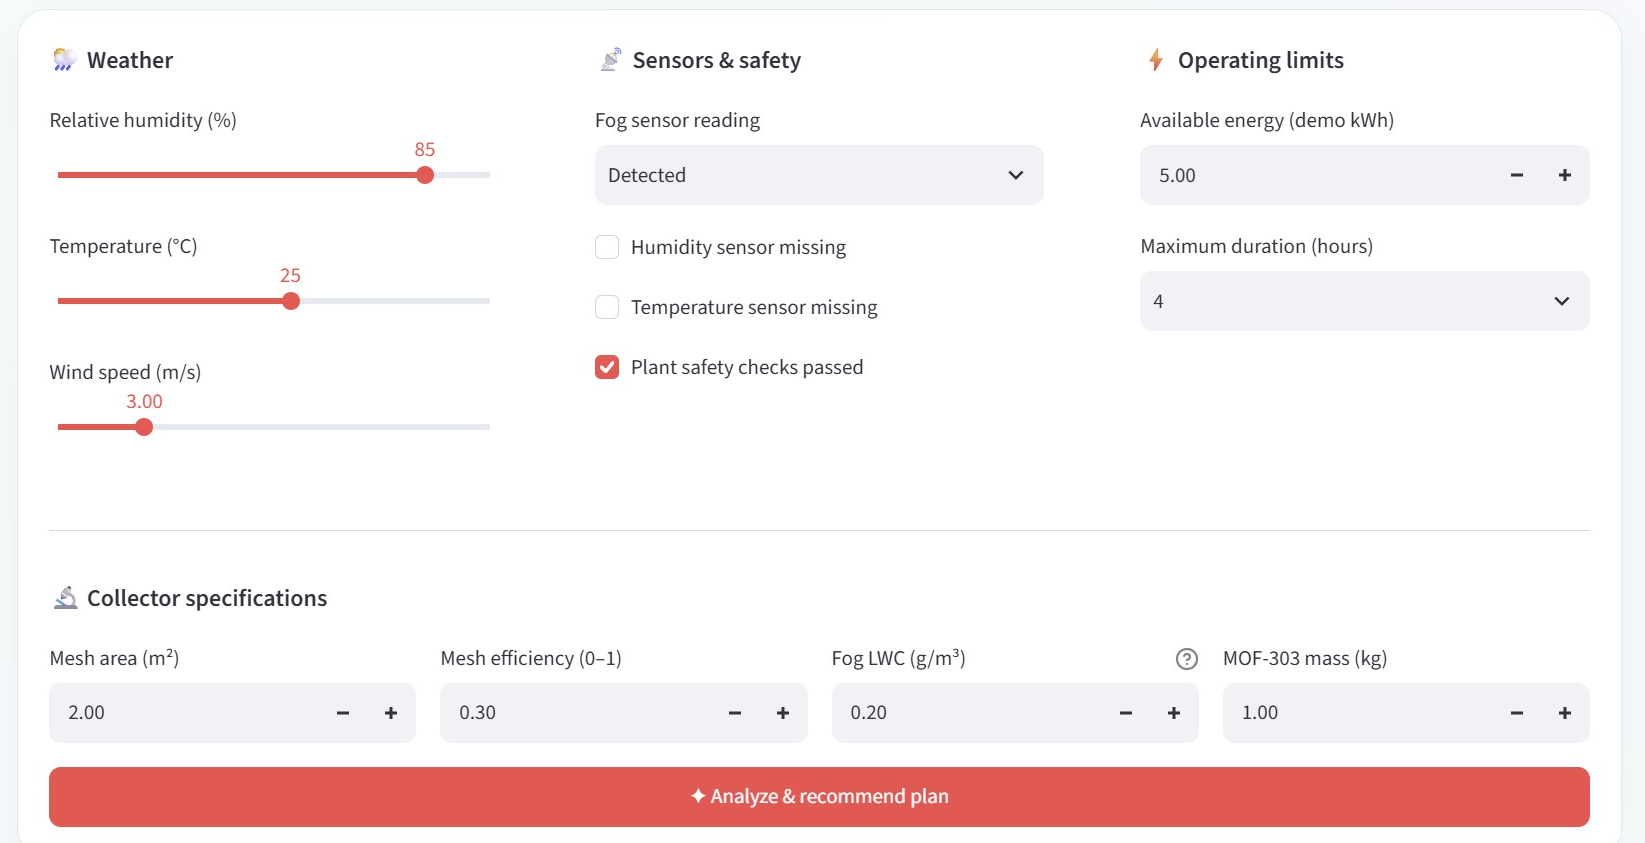
\includegraphics[width=\columnwidth]{figures/ui_inputs.png}
\caption{Input section of the AquaGent Streamlit page: weather, fog sensor and safety, operating limits and collector settings.}
\label{fig:ui}
\end{figure}

Behind the screen, one request goes through five steps:
\begin{enumerate}\setlength\itemsep{0pt}
\item \code{app.py} collects the values and creates an \code{Inputs} object.
\item \code{src/model.py} checks the values, and \code{src/uncertainty.py} estimates the chance of fog.
\item \code{src/csp.py} removes plans (collector, operating time) that are impossible or unsafe.
\item \code{src/decision.py} calculates the water and energy estimates, scores the valid plans and returns the recommendation with its reasons.
\item \code{app.py} shows the result, the operator approves or rejects it, and the run is saved in the session history, which can be exported as CSV.
\end{enumerate}
If the inputs are invalid, the process stops at step 2 with a warning. If no plan passes step 3, the page says that no feasible method exists and lists the broken constraints for each collector. In both cases the agent does not give a recommendation.

\twocolumn[{%
\subsection{System layers}
\vspace{2pt}
\begin{center}
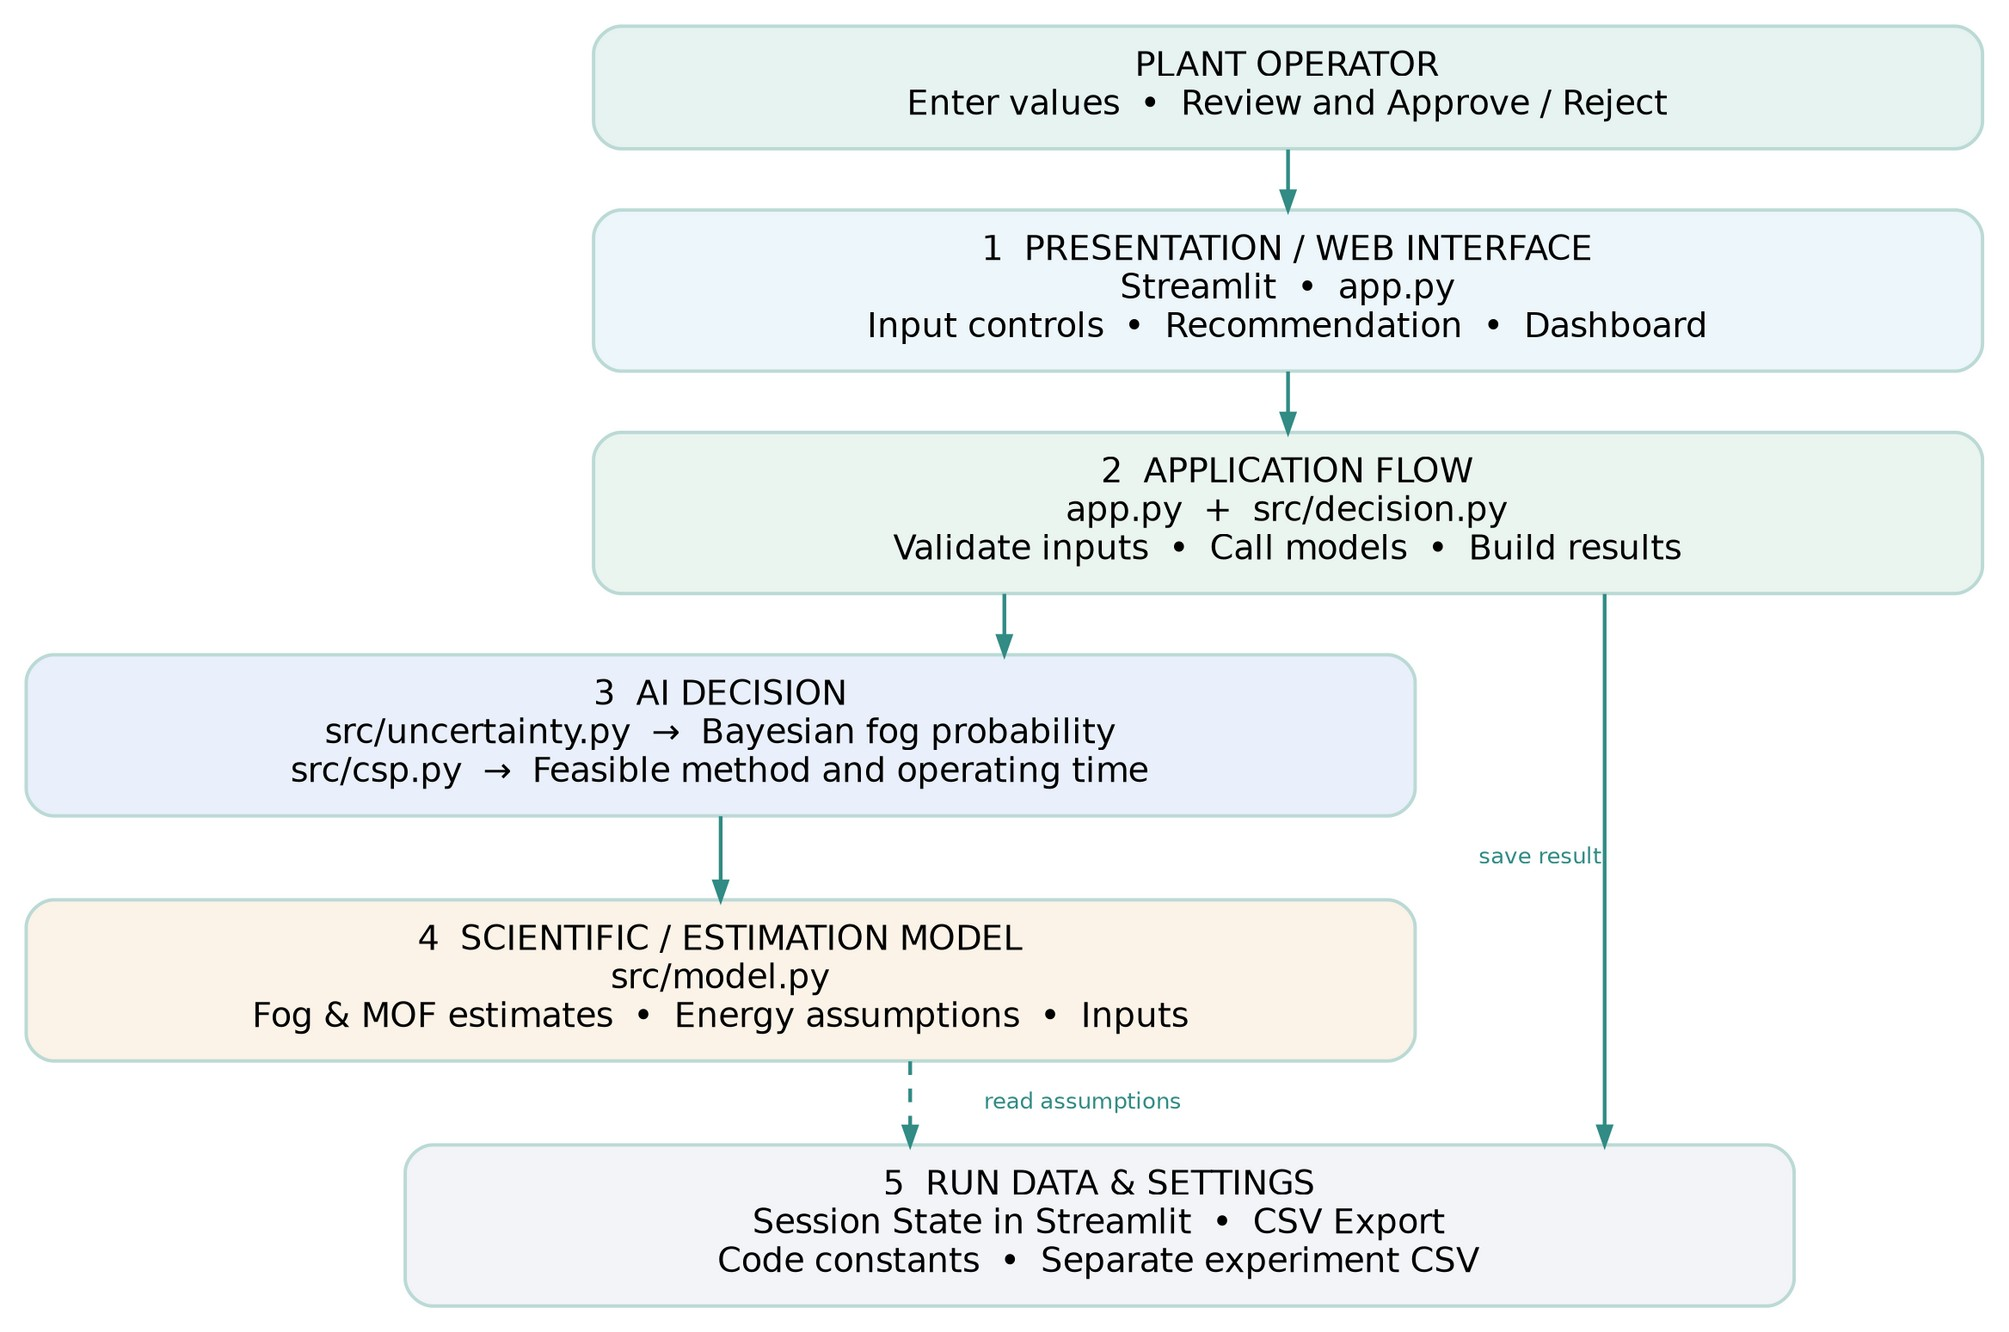
\includegraphics[width=0.92\textwidth]{figures/architecture.png}
\captionof{figure}{AquaGent system architecture with five logical layers. Some layers share a file (for example \code{app.py} is used by layers 1 and 2). There is no separate database and no real sensor connection in this prototype.}
\label{fig:arch}
\end{center}
\vspace{6pt}
}]
Figure~\ref{fig:arch} shows the five layers we used to organise the code.
\textbf{(1) Presentation:} the Streamlit \citep{streamlit} web page in \code{app.py}. It reads the inputs (Section~\ref{sec:ui}), shows the fog probability, the recommended plan and the water and energy estimates, and has Approve/Reject buttons.
\textbf{(2) Application flow:} \code{app.py} together with \code{src/decision.py}. It builds an \code{Inputs} object, checks the values, calls the models and collects the final result.
\textbf{(3) AI decision:} \code{src/uncertainty.py} computes the fog probability, \code{src/csp.py} finds the valid (method, hours) plans, and \code{src/decision.py} ranks them.
\textbf{(4) Scientific model:} \code{src/model.py} defines the inputs and calculates the simulated water and energy for fog and MOF-303.
\textbf{(5) Run data and settings:} the run history is kept in the Streamlit session and can be downloaded as CSV, and the demo constants are fixed in the code.
We use these layers only to explain the code; they do not run as separate services. Because the AI parts are in separate files, we could test each one alone, and a better MOF model can be added later without changing the web page.


% ---------------------------------------------------------------
\section{Methodology}

\subsection{Bayesian sensor model}
Let $F$ mean ``there is fog'', and let $E^{+}$ and $E^{-}$ mean the sensor says yes or no. We start with a prior $\pi=P(F)$, a sensitivity $s=P(E^+\mid F)$ and a specificity $c=P(E^-\mid\neg F)$. Using Bayes' rule:
\begin{align}
P(F\mid E^{+}) &= \frac{s\,\pi}{s\,\pi + (1-c)(1-\pi)}, \label{eq:bayes}\\
P(F\mid E^{-}) &= \frac{(1-s)\,\pi}{(1-s)\,\pi + c\,(1-\pi)}.
\end{align}
If there is no reading, the agent keeps $P(F)=\pi$ and shows a warning, instead of making up a reading. For the demo we used $\pi=0.35$ and $s=c=0.90$. We chose these values ourselves; they were not measured in Jeddah. With these values, a ``yes'' gives $P(F\mid E^+)=0.829$ and a ``no'' gives $0.057$.

\newpage
\subsection{CSP for possible plans}
Each plan has two variables: the method $M\in\{\text{Fog},\text{MOF}\}$ and the duration $H\in\{1,2,4,8\}$ hours. A plan is removed if it breaks any of these rules:
\begin{itemize}\setlength\itemsep{0pt}
\item \textbf{Safety:} the safety check must pass;
\item \textbf{Time:} $H\le h_{\max}$;
\item \textbf{Energy:} $H\cdot r_M \le E_{\text{budget}}$, with assumed rates $r_{\text{Fog}}=0.10$ and $r_{\text{MOF}}=1.20$\,kWh/h;
\item \textbf{Fog only:} $P(F\mid E)\ge\tau=0.75$, wind $>0$ and assumed liquid-water content (LWC) $>0$;
\item \textbf{MOF only:} RH $>0$, so there is some vapour.
\end{itemize}
The threshold $\tau$ connects the Bayesian part with the CSP, because fog is only allowed when the agent is confident enough about it. The solver uses backtracking: it sets $M$ first and then $H$, skips any duration above $h_{\max}$, and checks the rules when both variables have values. There are only 8 possible plans, but we still used backtracking so the search keeps working if we add more methods or durations later. For each method that has no valid plan, the agent lists the rules it broke, and this list is what the operator sees as the explanation.

\subsection{Water and energy estimates}
For a fog mesh with area $A$ (m$^2$), capture efficiency $\eta$, wind speed $v$ (m/s) and liquid-water content LWC (g/m$^3$), the expected water after $H$ hours is
\begin{equation}
L_{\text{fog}} = 3.6\cdot \text{LWC}\cdot v \cdot A\cdot \eta \cdot H \cdot P(F\mid E). \label{eq:fog}
\end{equation}
LWC$\cdot v\cdot A$ is in g/s, and multiplying by 3600\,s/h and dividing by 1000\,g/L gives the factor 3.6 for L/h. We multiply by $P(F\mid E)$ to get an expected value when fog is not certain. For MOF-303 we take the daily Death Valley result from \citet{song2023mof} and scale it to $H$ hours:
\begin{equation}
L_{\text{MOF}} = 0.210\cdot m_{\text{MOF}}\cdot H/24. \label{eq:mof}
\end{equation}
Equation~\ref{eq:mof} is a big simplification for a class project, because in a real device adsorption, heating and condensation are not linear and depend on humidity and temperature. Our default settings are $A=2$\,m$^2$, $\eta=0.30$, LWC $=0.20$\,g/m$^3$ and $m_{\text{MOF}}=1$\,kg.

\subsection{Ranking and operator approval}
Each valid plan $p$ gets a score. More water gives a higher score, and using more of the energy budget gives a lower score:
\begin{equation}
S(p)=\frac{L_p}{1+E_p/E_{\text{budget}}},\qquad E_{\text{budget}}>0. \label{eq:score}
\end{equation}
If two plans have the same score, the one that uses less energy is chosen. The operator sees the best plan, the other valid plans, the fog probability and why each method was rejected, and then clicks Approve or Reject. We picked $S$ as a simple way to compare plans and it should not be read as a real cost model. If an input is not valid the agent returns \code{SENSOR\_WARNING}, and if no plan is valid it returns \code{NO\_FEASIBLE\_METHOD}. In our evaluation both of these count as correct, safe answers.

\subsection{How we tested the agent}
We tested the agent in three ways. (i) \emph{Unit tests}: 45 tests for input checking, the Bayesian update, the rules, the water models and full decisions (\code{python -m unittest discover -s tests}). (ii) \emph{Scenarios}: ten fixed cases with normal inputs, missing or misleading sensor data, wrong inputs and broken rules (\code{experiments/run\_simulation.py}). (iii) \emph{Sensitivity sweeps}: we changed one input at a time around a reference case (RH 85\%, 22\,$^\circ$C, fog sensor says yes, 8\,kWh, $h_{\max}=4$\,h, wind 2\,m/s, default device settings). We changed wind, LWC, MOF mass, RH and energy budget, and we also plotted Eq.~\ref{eq:bayes} for different sensor sensitivities. A Python script runs the project's own functions, saves the results in CSV files, and draws all the graphs from these CSV files. We used Python, NumPy \citep{harris2020numpy} and Matplotlib \citep{hunter2007matplotlib}. The source code (AquaGent\_3), tests, scenario definitions, analysis script and CSV results are submitted with this report.

% ---------------------------------------------------------------
\newpage
\section{Experimental Results and Discussion}

\subsection{Unit tests and scenarios}
All 45 unit tests passed. Passing the tests tells us the code works as designed for these inputs. It does not tell us if the predictions are accurate. Table~\ref{tab:scen} and Figure~\ref{fig:scen} show the ten scenarios. Six gave a recommendation, two returned \code{NO\_FEASIBLE\_METHOD} (no energy; failed safety check), and two returned \code{SENSOR\_WARNING} (missing humidity; humidity of 120\%). We expected these four cases to give no plan, so they are correct results. We picked the ten scenarios by hand to test certain situations, so they should not be used to calculate an ``accuracy''.

\begin{table}[!ht]
\centering
\setlength{\tabcolsep}{3.7pt}
\begin{tabular}{@{}lclrr@{}}
\toprule
\textbf{Scenario} & $\boldsymbol{P(F)}$ & \textbf{Result} & \textbf{L} & \textbf{kWh} \\
\midrule
Fog detected      & 0.829 & Fog 4\,h & 2.865 & 0.4 \\
Fog absent        & 0.057 & MOF 4\,h & 0.035 & 4.8 \\
Sensor missing    & 0.350 & MOF 4\,h$^\dagger$ & 0.035 & 4.8 \\
Low RH (30\%)     & 0.057 & MOF 4\,h & 0.035 & 4.8 \\
No energy         & 0.829 & No plan & -- & -- \\
Unsafe            & 0.829 & No plan & -- & -- \\
Missing RH        & --    & Warning & -- & -- \\
RH = 120\%        & --    & Warning & -- & -- \\
Low sensitivity   & 0.748 & MOF 4\,h & 0.035 & 4.8 \\
Tight energy      & 0.829 & Fog 2\,h & 1.432 & 0.2 \\
\bottomrule
\end{tabular}
\caption{Scenario results (simulated). $^\dagger$With a ``fog sensor missing'' warning; the prior is used. ``Low sensitivity'' uses $s=0.55$ and ``Tight energy'' uses $E_{\text{budget}}=0.2$\,kWh.}
\label{tab:scen}
\end{table}

\begin{figure}[!ht]
\centering
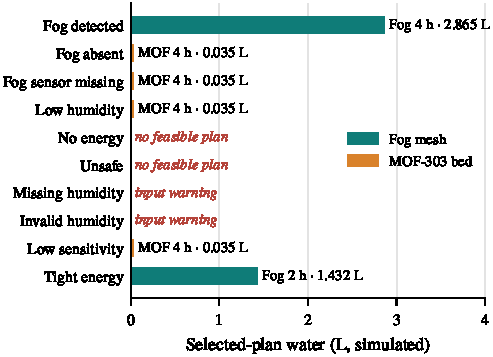
\includegraphics[width=\columnwidth]{figures/scenarios.pdf}
\caption{The chosen plan and simulated water for each scenario. An empty row means the agent gave no recommendation (it does not mean zero water).}
\label{fig:scen}
\end{figure}

Three of the scenarios show how the AI parts work together. In \textbf{Low sensitivity}, the sensor says there is fog, but because $s=0.55$ the probability is only 0.748, which is just under $\tau=0.75$. So the CSP removes fog and the agent chooses MOF. If we had just trusted the sensor's yes/no answer, fog would have been chosen even with an unreliable sensor. In \textbf{Sensor missing}, the agent uses the prior (0.35), warns the operator and does not pick fog. In \textbf{Tight energy}, 0.2\,kWh is not enough for even one hour of MOF (1.2\,kWh), and fog can only run for 2\,h. So with the same fog probability, the plan changed because energy was limited.

\subsection{Decision sensitivity: energy and sensor}
The last two scenarios above depend on the energy budget and on the sensor sensitivity, so we also changed these two inputs step by step around the reference case.

\begin{figure}[!ht]
\centering
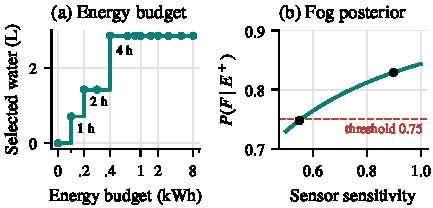
\includegraphics[width=\columnwidth]{figures/energy_posterior.pdf}
\caption{(a) Water of the chosen plan for different energy budgets. The steps happen when the CSP allows a longer fog run. (b) Fog probability after a ``yes'' reading for different sensor sensitivities (Eq.~\ref{eq:bayes}, $\pi=0.35$, $c=0.90$). The dots are the 0.55 and 0.90 scenarios.}
\label{fig:energy}
\end{figure}

\paragraph{Energy budget.} Figure~\ref{fig:energy}a shows what the CSP does. With 0\,kWh no plan is possible. With 0.1\,kWh the agent picks fog for 1\,h (0.716\,L), with 0.2--0.3\,kWh fog for 2\,h (1.432\,L), and with 0.4\,kWh or more fog for 4\,h (2.865\,L). After that the line stays flat up to 8\,kWh, because the 4\,h time limit does not allow longer runs. The result jumps in steps, which makes sense because hard rules are applied to a small set of choices.

\paragraph{Sensor reliability.} Figure~\ref{fig:energy}b shows that when $\pi=0.35$ and $c=0.90$, a ``yes'' reading only gets above $\tau=0.75$ if $s\ge 0.557$. Near this point, a small change in a sensor value that we assumed can change the decision. For this reason the sensitivity and specificity should be measured against real fog events before anyone relies on the threshold.

\twocolumn[{%
\subsection{Sensitivity of the water estimates}
\vspace{2pt}
\begin{center}
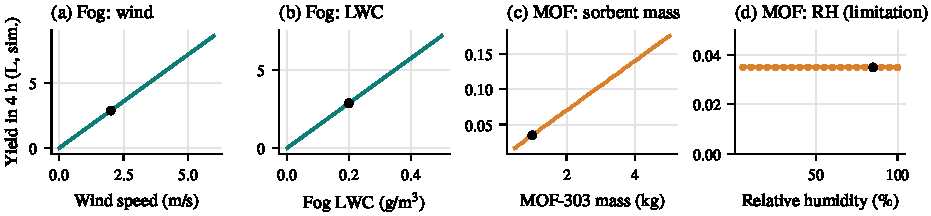
\includegraphics[width=\textwidth]{figures/sensitivity.pdf}
\captionof{figure}{Changing one input at a time around the reference case (black dot), for 4\,h runs. (a, b) Fog yield goes up in a straight line with wind and LWC because Eq.~\ref{eq:fog} is linear. (c) MOF yield goes up in a straight line with mass because of Eq.~\ref{eq:mof}. (d) MOF yield stays the same for all RH values. This flat line comes from a weakness in our model and does not describe real MOF behaviour.}
\label{fig:sens}
\end{center}
\vspace{6pt}
}]

\paragraph{Fog inputs.} When everything else stays the same, the expected 4\,h fog yield is 1.432, 2.865 and 5.729\,L at 1, 2 and 4\,m/s. LWC values of 0.10, 0.20 and 0.40\,g/m$^3$ give the same three numbers (Fig.~\ref{fig:sens}a,b). We get straight lines simply because our equation is linear. In real life, collection efficiency changes with wind speed, drop size and how wet the mesh is, so these lines should not be stretched far outside normal conditions.

\paragraph{MOF inputs.} MOF yield goes up in a straight line with mass: 0.035, 0.070 and 0.140\,L for 1, 2 and 4\,kg (Fig.~\ref{fig:sens}c). It stays at 0.035\,L for every RH from 5\% to 100\% (Fig.~\ref{fig:sens}d), because our model does not include an adsorption isotherm that depends on RH. In our opinion this is the biggest scientific weakness of the model. It is also the reason the ``Low RH'' scenario still chooses MOF.

\subsection{Discussion and limitations}
Overall, the decision logic worked the way we designed it. The Bayesian part changes whether fog is chosen, the CSP blocks unsafe or low-energy plans and says why, and the agent stops instead of guessing when the inputs are wrong. However, our results cannot show how much water a real device would make, how much energy it would use, how accurate the sensor is, whether the water is safe to drink, or whether Jeddah is a good place for this. Our main limitations are:
(1) the prior, sensitivity, specificity and $\tau$ are values we assumed;
(2) the fog equation is linear and uses an assumed LWC and efficiency;
(3) the MOF model is one daily field result scaled by hours, and humidity, temperature and cycling have no effect on it;
(4) the energy rates are example values, not measured heater or condenser loads;
(5) we chose the score $S$ ourselves, and the fog and MOF devices are not the same size (2\,m$^2$ vs.\ 1\,kg), so fog winning in our results comes from this setup and does not prove that one technology is better;
(6) all inputs are typed by hand and each decision is made separately.

% ---------------------------------------------------------------
\section{Conclusion and Future Work}

AquaGent combines two AI methods from our course into one agent that explains its choice. The Bayesian sensor model deals with the fact that fog cannot be seen directly. The backtracking CSP makes sure the safety, time and energy limits are followed. A simple score ranks the valid plans, and the operator always makes the last decision. All 45 tests passed, and the ten scenarios gave correct recommendations, correct refusals and correct input warnings. The sweeps also helped us find that our MOF model ignores humidity.

In the future we would like to: (1) replace the simple MOF rate with an adsorption isotherm that depends on RH and temperature, together with a cycle model; (2) collect local fog, wind and RH data in Jeddah to set the prior and sensor values, possibly with a dynamic Bayesian network; (3) measure the real energy use and water collected by both devices and use them to check the agent's decisions; (4) test the water quality before making any claim about drinking water; and (5) connect real sensors while still asking the operator to approve every action.

% ---------------------------------------------------------------
\newpage
\section*{Author Contributions}
Zainab Alameri and Abubaker Baobaid worked together on every part of this project and shared the work equally. Both authors carried out the literature review (Elicit search, DOI checks and the evidence table), designed and implemented the Bayesian sensor model, the backtracking CSP, the decision and ranking module, the water and energy formulas and the Streamlit interface, wrote the unit tests and scenarios, ran and checked the experiments, and wrote and reviewed all sections of this report. Each author signs the Contribution Declaration Form separately.

\section*{Use of AI Tools}
We used Elicit to search for papers. We also used a generative AI assistant (Claude) to help draft and edit the text of this report, to prepare the figures from our result files and to format the report in the ACL \LaTeX{} template. We reviewed the final report and take responsibility for its content.

\bibliography{references}

\end{document}
